\documentclass[a4paper]{IEEEtran} %tamaño del papel y el tipo de transcripción que será IEEE
\usepackage[utf8]{inputenc} %el tipo de codificación que incluye símbolos como la tilde
\usepackage[spanish]{babel} % hacemos que nuestro documentación vaya en español
\usepackage{cite} % citas bibliográficas
\usepackage{graphicx} %gráficos, usaremos solo .jpg o .png con estándares que ya veremos
\usepackage{subfigure}
\usepackage{url}
\usepackage{steinmetz}
\usepackage{amsmath}
\usepackage{booktabs} 
\providecommand{\keywords}[1]{\textbf{\textit{Términos Clave---}} #1}
\begin{document}
%\tableofcontents%tabla de contenidos
%\listoffigures%lista de figuras
\title{Control De Posición De Brazo Levitado Por Hélice}
\author{Quispe Condori Hanan Ronaldo}
\markboth{Teoría de Control I 2020-02-02}{} % Codigo del informe que corresponde a: semestre | mes | dia | numero de grupo con la G antepuesta | numero de proyecto con la P antepuesta | número de informe
\maketitle
\begin{abstract}
En este proyecto implementaremos el control de un brazo levitado por hélice, esto se logrará modificando la velocidad de giro de la hélice con el fin de que el brazo se encuentre en una posición deseada.
\end{abstract}

\section{Modelamiento Matemático}
\label{sec:modelamiento}

El modelo matemático de este sistema se logrará conectando el sistema del motor DC, sistema de propulsión de la hélice es el siguiente y el sistema del brazo. 

\begin{figure}[h]
    \centering
        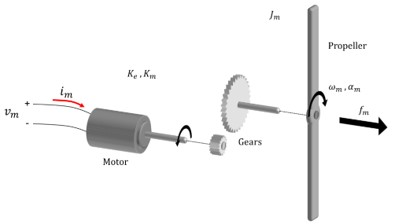
\includegraphics[width=8cm]{images/3}
        \caption{Diagrama sistema motor DC-hélice.}
        \label{fig:sistema_electrico}
\end{figure}

En el motor DC se tendrá.

\begin{figure}[h]
    \centering
        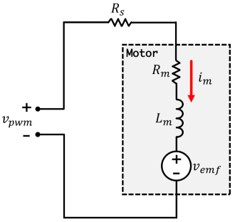
\includegraphics[width=5.5cm ,height=5cm]{images/2}
        \caption{Diagrama sistema motor DC-hélice.}
        \label{fig:motor DC}
\end{figure}

Usando la ley de voltajes de Kirchhoff se tendrá.

%Ecuación del motor. 
\begin{equation}
    \begin{split}
        -v_{pwm}+i_{m}R_{m}R_{s}+L_{m}\frac{di}{dt}-v_{emf}&=0\\
    \end{split}
    \label{eq:motor}
\end{equation}

Tendremos que a medida que transcurra el tiempo, el factor $\frac{di}{dt}\approx0$ por lo que la ecuación \ref{eq:motor} quedará.

\begin{equation}
    \begin{split}
        -v_{pwm}+i_{m}R_{m}R_{s}-v_{emf}&=0\\
    \end{split}
    \label{eq:motor1}
\end{equation}

Las ecuaciones para la fuerza de empuje de la hélice son \cite{edxpage1}.

\begin{equation}
    \begin{split}
        \tau_{m}&=K_{m}i_{m}(t)\\
        \tau_{m}&=J_{m}\alpha_{m}(t)\\
        f_{m}&=K_{t}\omega_{m}(t)^2\\
        v_{emf}&=K_{e}\omega_{m}(t)\\
    \end{split}
    \label{eq:helix}
\end{equation}

Donde 
\begin{itemize}
    \item $\tau_{m}$ es el torque ejercido por el motor.
    \item $\omega_{m}$ es la velocidad angular del motor.
    \item $\alpha_{m}$ es la aceleración angular de la hélice.
    \item $v_{emf}$ es el voltaje de retorno del motor.
    \item $K_{t}$ es el coeficiente de empuje de la hélice.
    \item $K_{m}$ es el coeficiente del torque del motor.
    \item $J_{m}$ es el momento de inercia del motor
\end{itemize}

Reemplazando \ref{eq:helix} en \ref{eq:motor1} y despejando $\alpha_{m}(t)$ se tendrá.

\begin{equation}
    \begin{split}
        \alpha_{m}(t)&=\frac{K_{m}}{J_{m}}\frac{v_{pwm}-K_{e}\omega_{m}(t)}{R_{s}+R_{m}}\\
    \end{split}
    \label{eq:motortork}
\end{equation}
Agregaremos un término de fricción correspondiente a la velocidad angular $-K_{f}\omega_{m}(t)$, en \ref{eq:motortork} se tendrá.

\begin{equation}
    \begin{split}
        \alpha_{m}(t)&=\frac{K_{m}}{J_{m}}\frac{v_{pwm}-K_{e}\omega_{m}(t)}{R_{s}+R_{m}}-K_{f}\omega_{m}(t)\\
    \end{split}
    \label{eq:motortork1}
\end{equation}

Donde $K_{f}$ es un coeficiente de fricción.
\vspace{5mm}

En el brazo se tendrá la siguiente ecuación apartir de la segunda ley de Newton.

\begin{figure}[h]
    \centering
        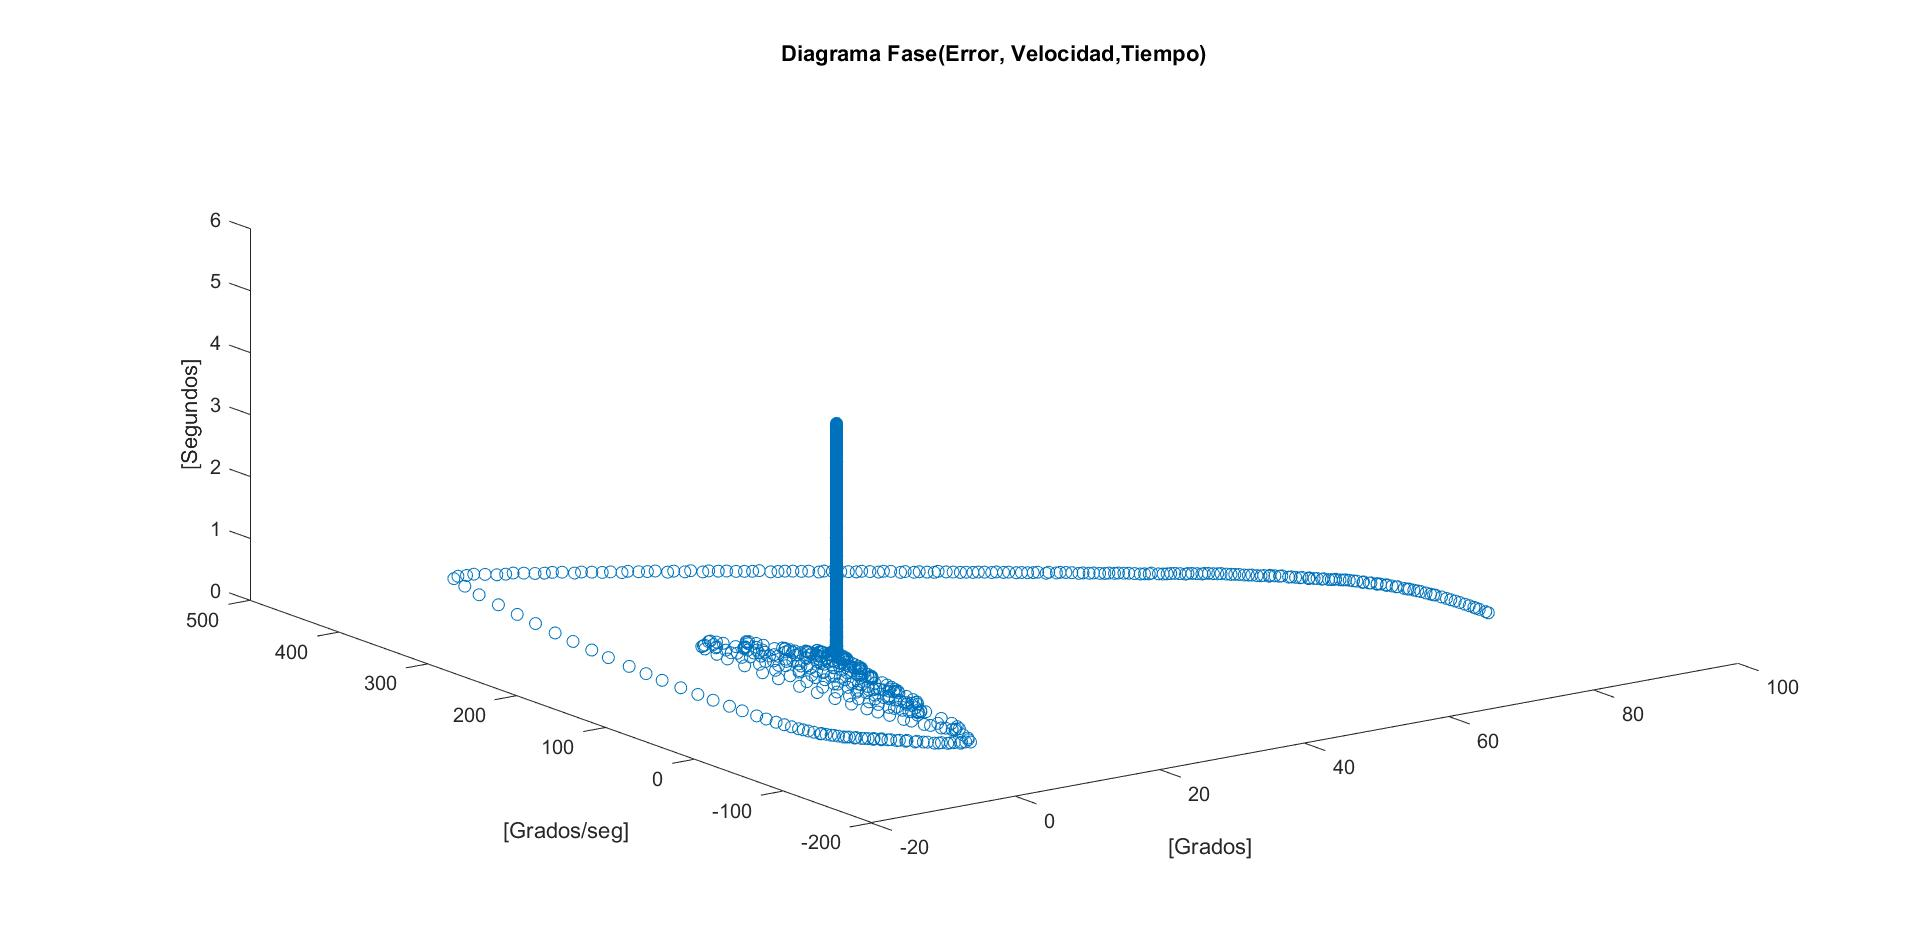
\includegraphics[width=6cm]{images/6.eps}
        \caption{Diagrama de cuerpo libre en el brazo.}
        \label{fig:DLC}
\end{figure}

\begin{equation}
    \begin{split}
        J_{a}\ddot{\theta}_{a}&=-mgcos(\theta_{a})+\tau_{a}\\
        \tau_{a}&=L_{a}f_{m}\\
        \ddot{\theta}_{a}&=-mgcos(\theta_{a})+f_{m}\frac{L_{a}}{J_{a}}\\
    \end{split}
    \label{eq:laplas}
\end{equation}

\section{Linealización de la Planta}

Haremos un cambio de coordenadas centrado en los puntos de equilibrio.

\begin{equation}
    \begin{split}
        \omega_{m}(t)&=\omega_{mo}+\partial\omega_{m}\\
        \theta_{m}(t)&=\theta_{mo}+\partial\theta_{m}\\
    \end{split}
    \label{eq:torkbrazo}
\end{equation}

Usando la expansión en series de Taylor y \ref{eq:torkbrazo} en la ecuación \ref{eq:laplas} se tendrá .

\begin{equation}
    \begin{split}
        \partial\ddot{\theta}_{m}(t)&=\frac{mg}{J_{a}}sen(\theta_{mo})\partial\theta_{a}+\frac{L_{a}}{J_{a}}2K_{t}\omega_{mo}\partial\omega_{m}\\
    \end{split}
    \label{eq:linealizada1}
\end{equation}
%\vspace{5mm}

Haciendo el mismo procedimiento en \ref{eq:motortork1} se tendrá.

\begin{equation}
    \begin{split}
        \partial\dot{\omega}_{m}(t)&=(\frac{-K_{m}K_{e}}{J_{m}(R_{s}+R_{m})}-K_{f})\partial\omega_{m}+\frac{K_{m}}{J_{m}(R_{s}+R_{m})}\partial v_{pwm}\\
    \end{split}
    \label{eq:linealizada2}
\end{equation}
\vspace{1mm}

Para simplificar el álgebra se harán los siguientes cambios de variable.

\begin{equation}
    \begin{split}
        A&=\frac{K_{m}K_{e}}{J_{m}(R_{s}+R_{m})}+K_{f}\\
        B&=\frac{K_{m}}{J_{m}(R_{s}+R_{m})}\\
        C&=\frac{mg}{J_{a}}sen(\theta_{mo})\\
        D&=\frac{L_{a}}{J_{a}}2K_{t}\omega_{mo}\\
    \end{split}
    \label{eq:consideraciones}
\end{equation}


Haciendo $\partial v_{pwm}=\partial \mu$ en \ref{eq:linealizada1}; Reemplazando \ref{eq:consideraciones} en \ref{eq:linealizada1} y \ref{eq:linealizada2} y usando la transformada de Laplace se tendrá.

\begin{equation}
    \begin{split}
        s\Delta\omega_{m}(s)&=-A\Delta\omega_{m}(s)+B\Delta\mu(s)\\
        \Delta\omega_{m}(s)(s+A)&=B\Delta\mu(s)\\
        \frac{\Delta\omega_{m}(s)}{\Delta\mu(s)}&=\frac{B}{s+A}\\
        s^2\Delta\theta_{a}(s)&=C\Delta\theta_{a}(s)+D\Delta\omega_{m}(s)\\
        \Delta\theta_{m}(s)(s^2-C)&=D\Delta\omega_{m}(s)\\
        \frac{\Delta\theta_{a}(s)}{\Delta\omega_{m}(s)}&=\frac{D}{s^2-C}\\
        \frac{\Delta\theta_{a}(s)}{\Delta\omega_{m}(s)}\frac{\Delta\omega_{m}(s)}{\Delta\mu(s)}&=\frac{B}{s+A}\frac{D}{s^2-C}\\
        \frac{\Delta\theta_{a}(s)}{\Delta\mu(s)}&=\frac{\Delta\theta_{a}(s)}{\Delta v_{pwm}(s)}\\
        \frac{\Delta\theta_{a}(s)}{\Delta v_{pwm}(s)}&=\frac{BD}{(s+A)(s^2-C)}\\
    \end{split}
    \label{eq:linealfin1}
\end{equation}
\section{Sensibilidad del sistema}
$Im+Re$Se calculará la sensibilidad a variaciones de la masa, en $C$ se hará $C=mc'$, donde $c'=\frac{g}{J_{a}}sen(\theta_{mo})$.
Para Lazo Abierto
\begin{equation}
    \begin{split}
        S_m^T&=\frac{\frac{dT}{T}}{\frac{dm}{m}}\\
        T&=\frac{BD}{(s+A)(s^2-mc')}\\
        \frac{dT}{T}&=\frac{sc'm}{(s+A)(s^2-mc')}\frac{dm}{m}\\
        S_m^T&=\frac{sc'm}{(s+A)(s^2-mc')}\\
        S_m^T&=\frac{sC}{(s+A)(s^2-C)}\\
    \end{split}
    \label{eq:m_sensi}
\end{equation}

Para Lazo Cerrado
\begin{equation}
    \begin{split}
        S_m^T&=\frac{\frac{dT}{T}}{\frac{dm}{m}}\\
        T&=\frac{BD}{BD+(s+A)(s^2-mc')}\\
        \frac{dT}{T}&=\frac{sc'm}{BD+(s-A)(s^2-mc')}\frac{dm}{m}\\
        S_m^T&=\frac{sc'm}{BD+(s+A)(s^2-mc')}\\
        S_m^T&=\frac{sC}{BD+(s+A)(s^2-C)}\\
    \end{split}
    \label{eq:m_sensiclose}
\end{equation}

\section{diagrama de polos y ceros}
Del denominador de la función de transferencia se tienen 3 polos, en $A$, $\sqrt{C}$ y $\sqrt{-C}$

\begin{figure}[h]
    \centering
        \includegraphics[width=8cm]{images/polos_ceros.eps}
        \caption{Diagrama de Polos y Ceros.}
\end{figure}

El sistema es inestable.
\section{error de estado estacionario}
El sistema es inestable, por eso no se podrá calcular el error de estado estacionario para este sistema.
\section{Análisis de estabilidad}
El denominador se expandirá de la siguiente manera
\begin{equation}
    \begin{split}
        T&=\frac{BD}{s^3+s^2A+s(-C)-AC+BD}\\
    \end{split}
    \label{eq:m_sensiclose}
\end{equation}
\subsection{Criterio de Routh}
\begin{figure}[h]
    \centering
        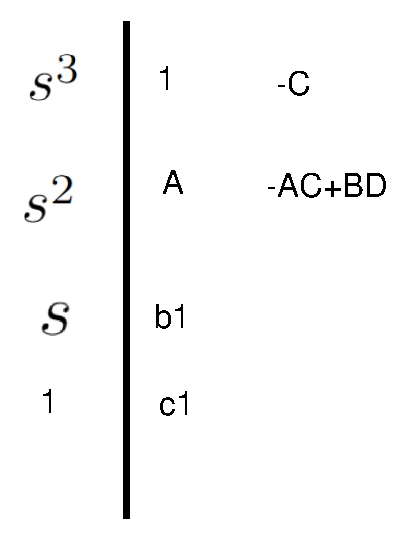
\includegraphics[width=3cm]{images/routh.eps}
        \caption{Arreglo de Routh.}
\end{figure}

\begin{equation}
    \begin{split}
        b1&=\frac{-AC+AC-DB}{A}=\frac{-DB}{A}\\
    \end{split}
    \label{eq:routh1}
\end{equation}

\begin{equation}
    \begin{split}
        c1&=-AC+DB\\
    \end{split}
    \label{eq:routh1}
\end{equation}

Vemos que existe un cambio de variable, el sistema es inestable.

\subsection{Criterio de Hurwitz}

\begin{equation}
    \begin{split}
        \Delta_1&=a_2=A>0\\
        \Delta_2&=det(
        \begin{matrix}
            a_2 & a_0 \\
            a_3 & a_1 \\
        \end{matrix})=
        -AC+AC+BD=DB>0\\
        \Delta_3&=det(
        \begin{matrix}
            a_2 & a_0 & 0 \\
            a_3 & a_1 & 0 \\
            0 & a_2 & a_0 \\
        \end{matrix})=A(-C)-(-AC+BD)=-BD\\
    \end{split}
    \label{eq:hurwitz}
\end{equation}

No todos los determinates son positivos, el sistema es 
inestable.

\section{Lugar Geométrico de las Raices}
Por simple inspección de los polos de la función de transferencia calculada en \ref{eq:linealfin1} podemos ver que el sistema es inestable ya que posee un polo en $s=\sqrt{C}$, grafiquemos el lugar geométrico de las raices para este sistema

Procederemos a calcular la función de transferencia en lazo cerrado.
\begin{equation}
    \begin{split}
        T&=\frac{G_{c}G_{p}}{1+G_{c}G_{p}}\\
    \end{split}
    \label{eq:locus}
\end{equation}

Donde 
\begin{itemize}
    \item $G_{c}$ es el controlador a usar, para la gráfica del lugar geométrico de las raices, este será una constante.
    \item $G_{p}$ es la función de transferencia de la planta en lazo abierto calculada en \ref{eq:linealfin1}
\end{itemize}

Haciendo $G_{c}=k$ en el denominador se tendrá.
\begin{equation}
    \begin{split}
        1+kG_{p}&=0\\
        kG_{p}&=-1\\
        |kG_{p}|&=1\\
        \phase{kG_{p}}&=\pi\\
    \end{split}
    \label{eq:locus_mano}
\end{equation}
Usando \ref{eq:locus_mano} y las demas reglas descritas en  \cite{dorf2005sistemas}, se tendrá el siguiente gráfico.
%$-A-\sqrt{C}+\sqrt{C}$ 
\begin{figure}[h]
    \centering
        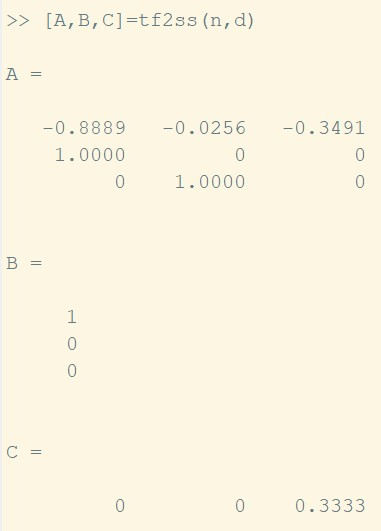
\includegraphics[width=8cm]{images/7.eps}
        \caption{Lugar Geométrico de las Raices.}
        \label{fig:locus}
\end{figure}

Del gráfico podemos observar lo siguiente

\begin{itemize}
    \item Existen tres polos por lo que tendremos el mismo número de ramas.
    \item El origen de las asintotas es en el punto $\frac{-A}{3}$
    \item Los angulos de estas rectas asintotas son $\frac{\pi}{3},\frac{-\pi}{3},-\pi$, este esta dado por la fórmula $\frac{(2k+1)\pi}{3}$
\end{itemize}

El gráfico del lugar geométrico de las raices nos dice que el control proporcional no nos servirá para hacer nuestro sistema estable, mas cabe mencionar que la posición de los polos dependerá de los puntos de equilibrio elegidos según sea la aplicación deseada. 

\section{Diseño del Controlador}

Usaremos un control PID para hacer nuestro sistema estable, con este fin se tendrá.

\begin{equation}
    \begin{split}
        G_{c}&=k_{p}+sk_{d}+k_{i}\\
    \end{split}
    \label{eq:PD}
\end{equation}
Reemplazando \ref{eq:PD} en \ref{eq:locus} se tendrá
\begin{equation}
    \begin{split}
        T&=\frac{BD(k_{i}+sk_{p}+s^2k_{d})}{s^4+As^3+(k_{d}BD-C)s^2+s(BDk_{p}-AC)+BDk_{i}}\\
    \end{split}
    \label{eq:PD1}
\end{equation}

Para simplificar el algebra se usarán valores conocidos de las constantes mencionados en \ref{eq:PD1} y se elegirán puntos de equilibrio para las mismas \cite{dcmotor},\cite{edxpage}.
%\vspace{2mm}
\begin{itemize}
    \item $sen(\theta_{mo})=0$
    \item $K_{m}=0.0053$
    \item $K_{3}=0.0053$
    \item $J_{m}=3\times 10^-6$
    \item $J_{a}=4.5\times 10^-4$
    \item $R_{s}=0.5$
    \item $R_{m}=0.5$
    \item $L_{a}=0.15$
\end{itemize}

Usando estos valores, se tendrán el valor de las constantes
\begin{equation}
    \begin{split}
        A&=11.473\\
        B&=1766.667\\
        C&=0\\
        D&=8.18\\
    \end{split}
    \label{eq:considera_numerica}
\end{equation}

Se puede observar que el valor de $C=0$ hace que el sistema pase de ser inestable a marginalmente estable, esto hace que el sistema sea oscilante mas no estable.

Reemplazando \ref{eq:considera_numerica} en \ref{eq:PD1} se tendrá.

\begin{equation}
    \begin{split}
        \frac{14451.336(k_{i}+sk_{p}+s^2k_{d})}{s^4+11.473s^3+k_{d}14451.336s^2+s14451.336k_{p}+14451.336k_{i}}\\
    \end{split}
    \label{eq:PD_numerica}
\end{equation}

\ref{eq:PD_numerica} posee 4 polos que podremos manipular cambiando $k_{i},k_{p},k_{d}$, ya que no fueron especificados los parametros de repuesta en transitorio ni condiciones de operación del sistema, podemos elegir cualquier punto o puntos en el semiplano negativo donde nuestro sistema será estable, el polo elegido será $s=-2.868$ 

Bajo esta premisa en el denominador de \ref{eq:PD_numerica} se cumplira que:
\begin{equation}
    \begin{split}
        s^4+11.473s^3+k_{d}14451.336s^2+s14451.336k_{p}\\+14451.336k_{i}=\\s^4+11.473s^3+\frac{1542267}{31250}s^2+s\frac{368601813}{3906250}+\frac{264287499921}{3906250000}\\
    \end{split}
    \label{eq:PD_numerica1}
\end{equation}

De aqui se obtendrán los valores de $k_{i},k_{p},k_{d}$

\begin{equation}
    \begin{split}
        k_{i}&=4.682\times 10^-3\\
        k_{p}&=6.53\times 10^-3\\
        k_{d}&=3.415\times 10^-3\\
    \end{split}
    \label{eq:vieta}
\end{equation}

Se usará Simulink para simular este sistema
\begin{figure}[h]
    \centering
        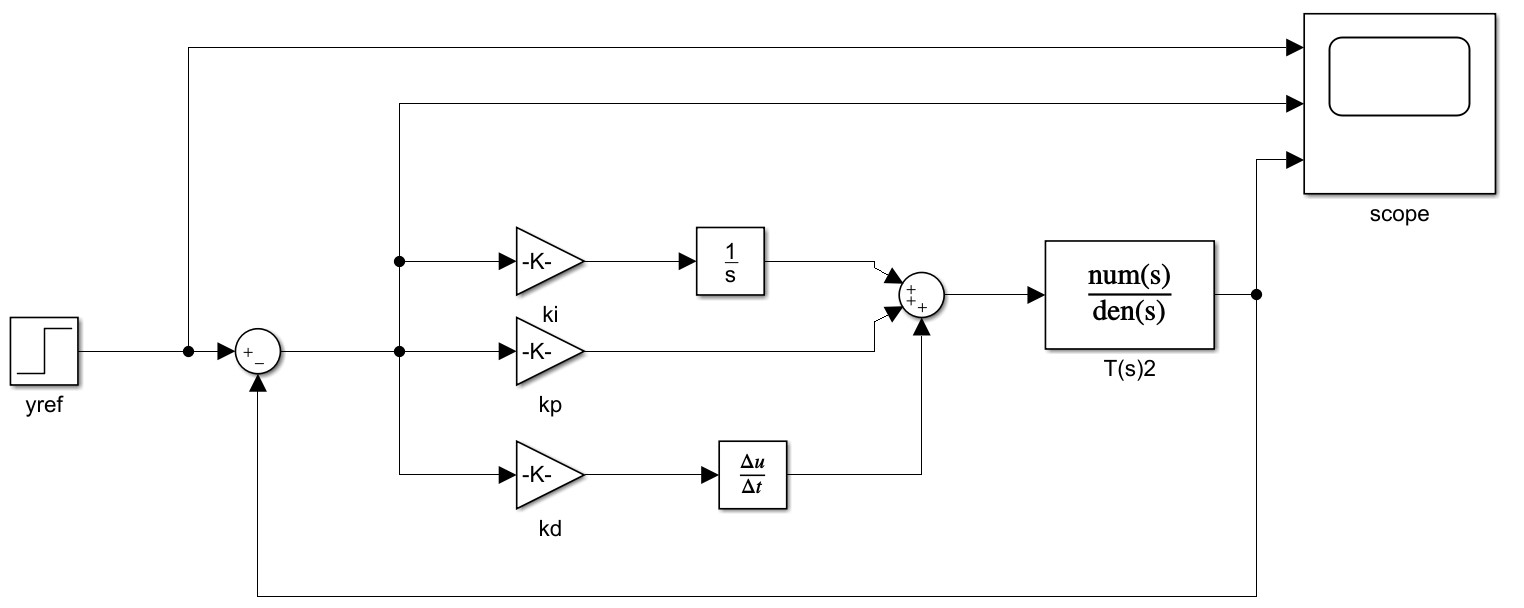
\includegraphics[width=8cm]{images/8}
        \caption{Diagrama de Bloques}
        \label{fig:simu}
\end{figure}
\vspace{100mm}

La configuración de los bloques es la siguiente

\begin{figure}[h]
    \centering
        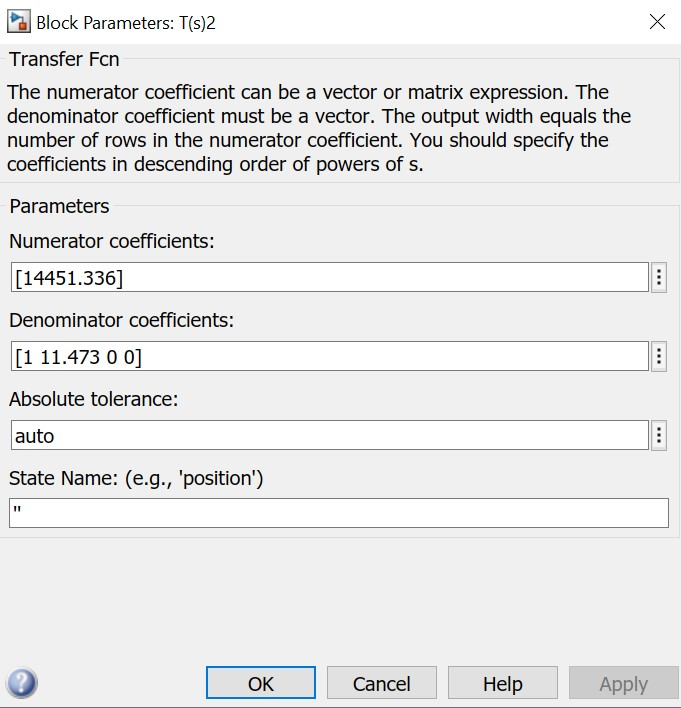
\includegraphics[width=5cm]{images/9}
        \caption{Función de Transferencia}
        \label{fig:config1}
\end{figure}

%\vspace{10mm}

\begin{figure}[h]
    \centering
        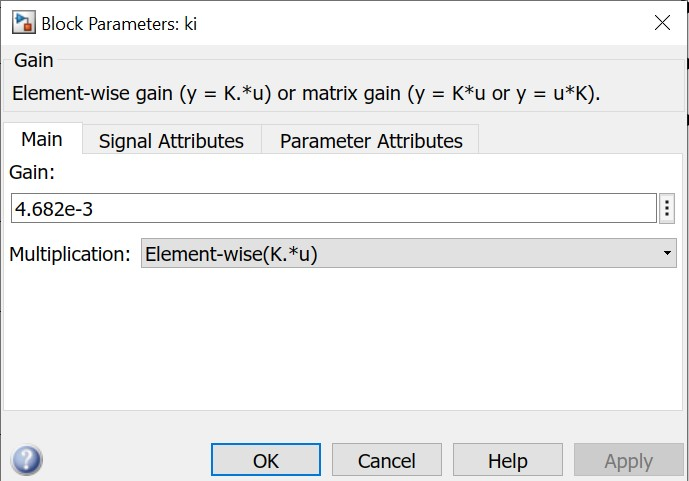
\includegraphics[width=5cm]{images/10}
        \caption{Ganancia del Integrativo.}
        \label{fig:config2}
\end{figure}

\begin{figure}[h]
    \centering
        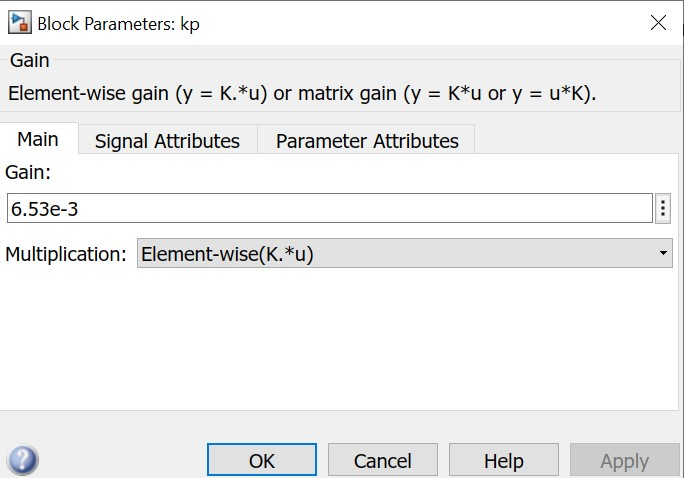
\includegraphics[width=5cm]{images/11}
        \caption{Ganancia del Proporcional.}
        \label{fig:config3}
\end{figure}

\begin{figure}[h]
    \centering
        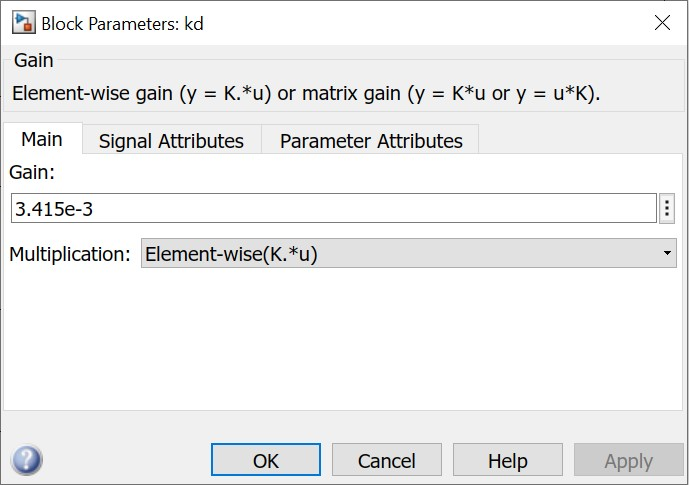
\includegraphics[width=5cm]{images/12}
        \caption{Ganancia del Derivativo.}
        \label{fig:config4}
\end{figure}
\vspace{20mm}
La respuesta al escalon es la siguiente
\begin{figure}[h]
    \centering
        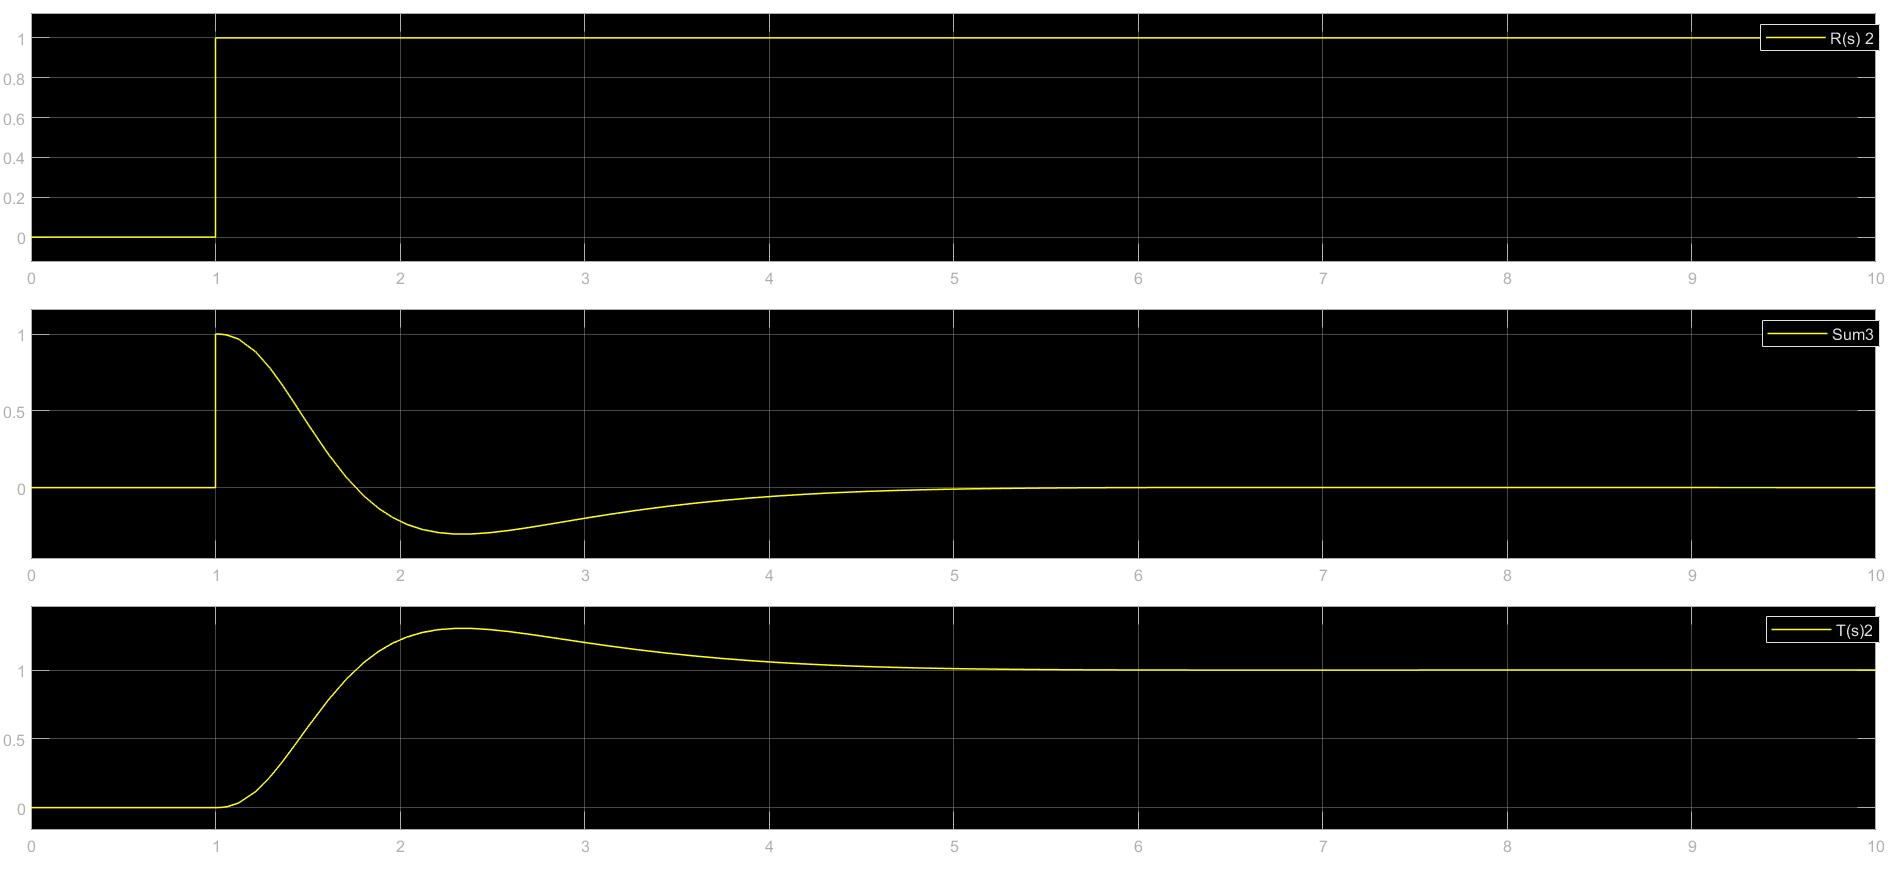
\includegraphics[width=9cm, height=9cm]{images/13}
        \caption{Respuesta al Escalon.}
        \label{fig:result}
\end{figure}

De esta simulación se obtienen los siguientes datos
\begin{itemize}
    \item El tiempo de pico es de $2.296seg$
    \item El tiempo de subida es de $1.762seg$
    \item El tiempo de asentamiento es de $4.89seg$
    \item El valor pico es de $1.302$
    \item La sobreelongación es de $0.302$
\end{itemize}   
\section{Respuesta en Frecuencia}
Se obtuvo la siguiente ecuación que representa al sistema + controlador

\begin{equation}
    \begin{split}
        \frac{14451.336(k_{i}+sk_{p}+s^2k_{d})}{s^4+11.473s^3+k_{d}14451.336s^2+s14451.336k_{p}+14451.336k_{i}}\\
    \end{split}
    \label{eq:PD_num}
\end{equation}

Reemplazando los valores para las ganancias se tiene
\begin{equation}
    \begin{split}
        \frac{14451.336(4.682\times 10^{-3}+s6.653\times 10^{-3}+s^2 3.415\times 10^{-3})}{(s+2.868)^4}\\
    \end{split}
    \label{eq:PD_num_reeempla}
\end{equation}

Hagamos un analisis de bode para esta nueva función de transferencia
\vspace{60mm}
\begin{figure}[h]
    \centering
        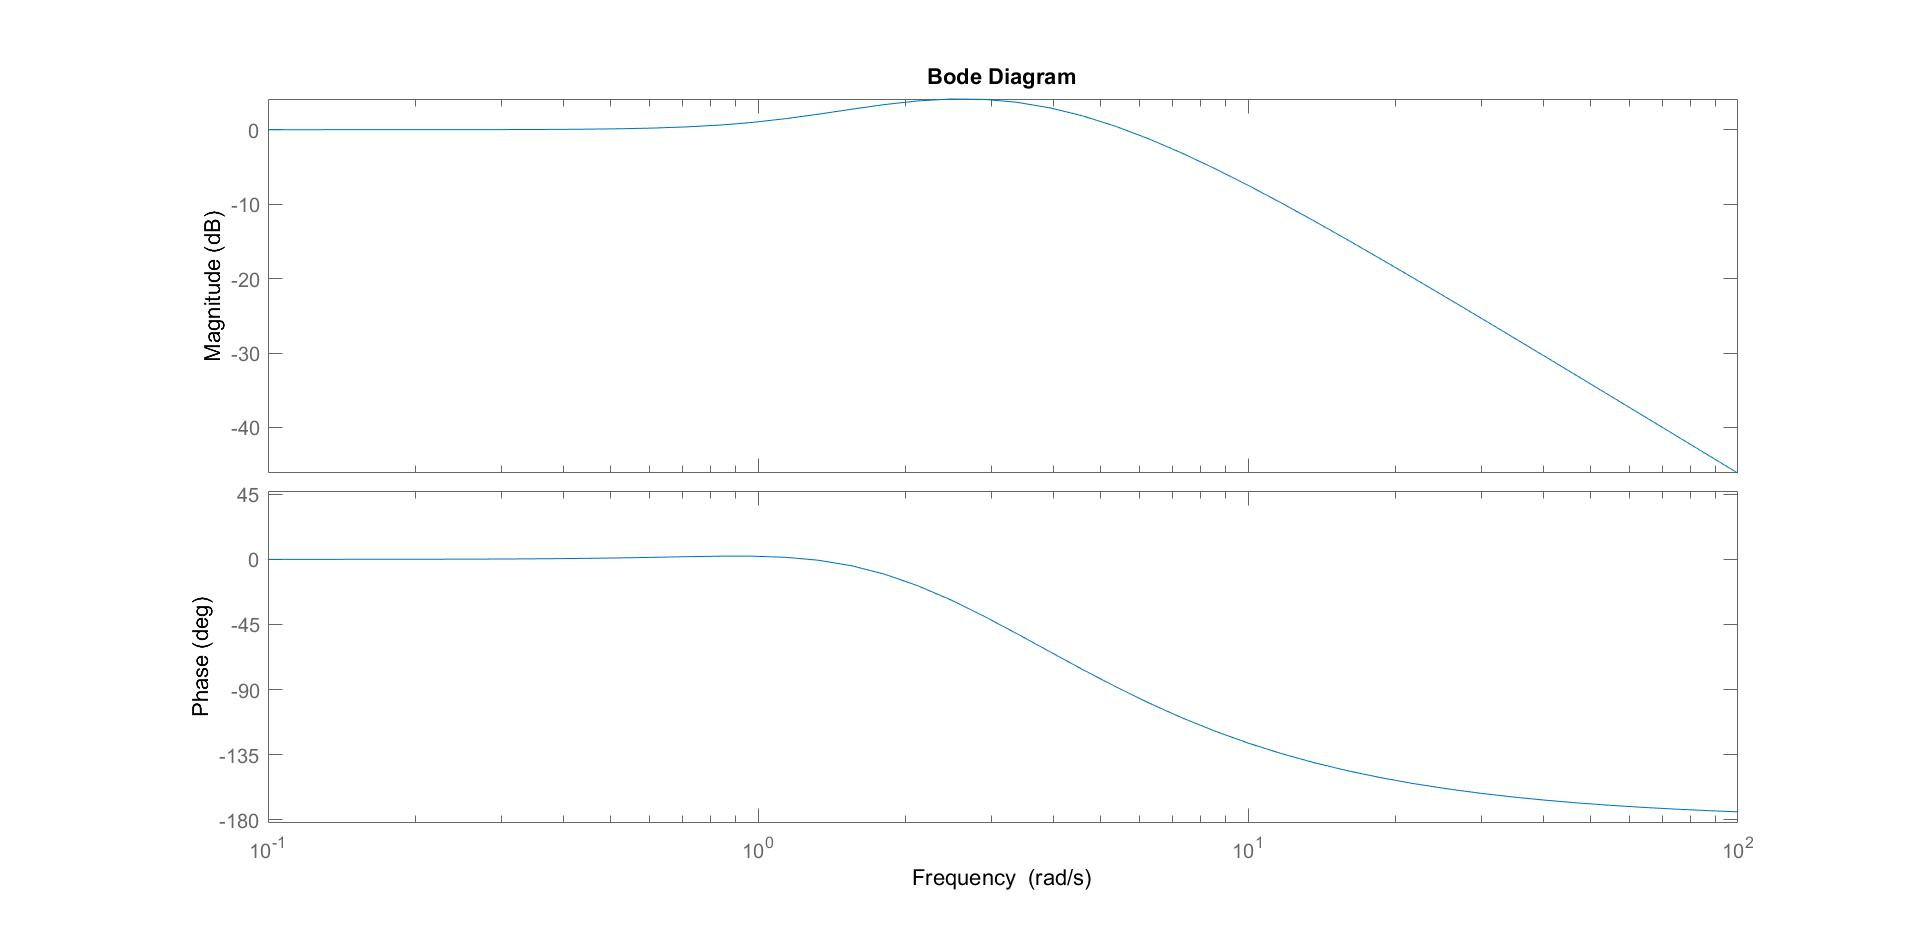
\includegraphics[width=9cm]{images/14}
        \caption{Diagrama de Bode Sistema y Controlador.}
        \label{fig:bode}
\end{figure}

Podemos observar que:

\begin{itemize}
    \item El sistema en la magnitud, atenuara las entradas por encima de su frecuencia de corte al igual que un filtro pasabajos.
    \item El sistema en la fase, atrasará la salida con respecto a la entreada a frecuencias por encima de su frecuencia de corte.
    \item El ancho de banda es de 7.2518  
\end{itemize}

El diagrama de bode del sistema sin controlador es el que sigue.

\begin{figure}[h]
    \centering
        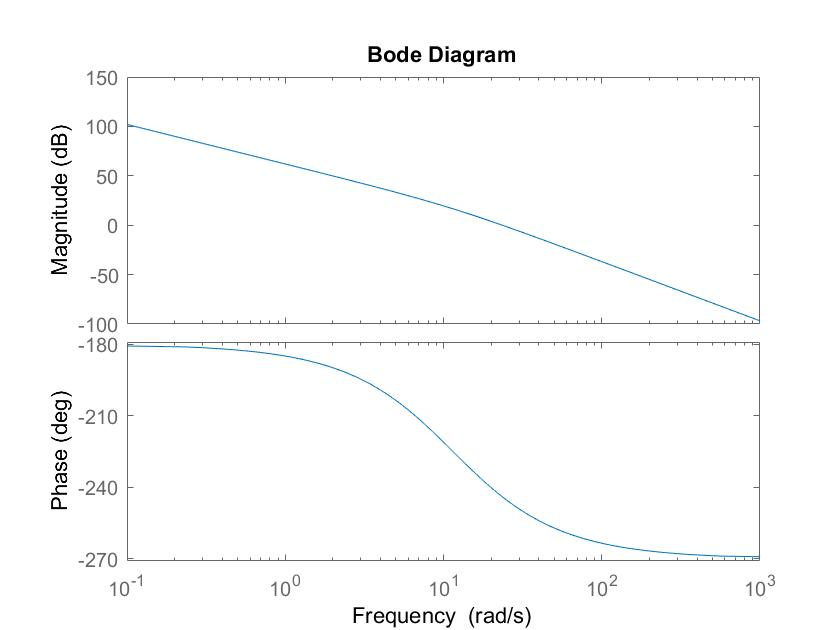
\includegraphics[width=9cm,height=5cm]{images/15}
        \caption{Diagrama de Bode Sistema sin Controlador.}
\end{figure}

\begin{itemize}
    \item La ganancia en DC es infinita, por ello el ancho de banda es indeterminado.
    \item A frecuencias bajas el sistema invertira la fase de la entrada y a frecuencias altas adelantará la salida en noventa grados con respecto a la entrada.
\end{itemize}

\section{Conclusiones y Observaciones}
\begin{itemize}
    \item Los criterios de Routh y Hurwitz se complementan confirmando que el sistema no es estable.
    \item Al observar el cambio en la respuesta en el tiempo se puede concluir la efectividad del sistema de control PID para nuestro sistema.
    \item Se pudo comprobar la predicción del metodo del lugar de las raices al elegir valores numéricos para las constantes.
    \item Se pudo observar nuestro sistema actua como un filtro pasabajos.
    \item Se pudo obsevar el efecto simplificador de la linealización del sistema usando la expansión en series de Taylor.
\end{itemize}
\bibliographystyle{ieeetr}
\bibliography{bibliografia}
\end{document}
